%%%% PGCT submission draft in the IJCAI-27 template (ijcai27.sty, named.bst from the official author kit).
%%%% Intended engine: pdfLaTeX (e.g. Overleaf). The \pdfinfo shim below only matters for XeTeX/Tectonic builds.
\documentclass{article}
\pdfpagewidth=8.5in
\pdfpageheight=11in

\usepackage{ijcai27}

\usepackage{times}
\usepackage{soul}
\usepackage{url}
\usepackage[hidelinks]{hyperref}
\usepackage[utf8]{inputenc}
\usepackage[small]{caption}
\usepackage{graphicx}
\usepackage{amsmath}
\usepackage{amsthm}
\usepackage{booktabs}
\usepackage{algorithm}
\usepackage{algorithmic}
\usepackage[switch]{lineno}
\usepackage{amssymb}
\usepackage{xcolor}
\usepackage{tikz}
\renewcommand{\algorithmicrequire}{\textbf{Input:}}
\renewcommand{\algorithmiccomment}[1]{\hfill$\triangleright$~#1}
% Local XeTeX/Tectonic builds only: metric-compatible Times/Helvetica clones. pdfLaTeX skips this block.
\ifdefined\XeTeXrevision\usepackage{fontspec}
  \setmainfont{texgyretermes}[Extension=.otf,UprightFont=*-regular,BoldFont=*-bold,ItalicFont=*-italic,BoldItalicFont=*-bolditalic]
  \setsansfont{texgyreheros}[Extension=.otf,UprightFont=*-regular,BoldFont=*-bold,ItalicFont=*-italic,BoldItalicFont=*-bolditalic]\fi

% Comment out this line in the camera-ready submission
\linenumbers

\urlstyle{same}

% Shared colours and TikZ styles for the PGCT papers and slides (requires tikz, xcolor).
\usetikzlibrary{arrows.meta,positioning,calc,fit,backgrounds,shapes.geometric}
\definecolor{pgblue}{HTML}{1F4E9A}
\definecolor{pgsky}{HTML}{DCE7F7}
\definecolor{pgorange}{HTML}{C0504D}
\definecolor{pgsand}{HTML}{FBE9DA}
\definecolor{pggreen}{HTML}{2E7D4F}
\definecolor{pgmint}{HTML}{E2F2E8}
\definecolor{pggrey}{HTML}{6B6B6B}
\definecolor{pglight}{HTML}{F4F4F4}
\tikzset{
  pg/.style={font=\sffamily\small},
  stage/.style={draw=pgblue,line width=.8pt,rounded corners=3pt,fill=white,align=center,
                minimum height=1.25cm,text width=2.7cm,inner sep=3pt},
  card/.style={draw=pggrey,rounded corners=2pt,fill=white,align=center,inner sep=2.5pt,font=\sffamily\scriptsize},
  box/.style={draw=pgblue,line width=.8pt,rounded corners=3pt,fill=white,align=center,inner sep=4pt},
  flow/.style={-{Stealth[length=2.4mm]},line width=.9pt,draw=pgblue},
  flowg/.style={-{Stealth[length=2.2mm]},line width=.8pt,draw=pggrey},
  flowo/.style={-{Stealth[length=2.4mm]},line width=.9pt,draw=pgorange},
  band/.style={rounded corners=5pt,inner sep=7pt},
  num/.style={circle,fill=pgblue,text=white,font=\sffamily\bfseries\scriptsize,inner sep=1.2pt,minimum size=4mm},
  lbl/.style={font=\sffamily\scriptsize,text=pggrey,align=center},
}
\newcommand{\stagetitle}[1]{{\bfseries\color{pgblue}#1}}

% Shared verbatim by the English and Korean manuscripts. Numbers follow invocation order.
\newcommand{\ModelEquation}{\begin{equation}\label{eq:model}
 \widehat r_i(q;\psi_i)=\operatorname{MLP}_{\psi_i}
 (u_t,e_{a_t+1},u_{t+1}),\quad u_t=P(o_{i,t}).
\end{equation}}
\newcommand{\RewardLossEquation}{\begin{equation}\label{eq:rloss}
 \mathcal L_i^r(\psi_i)=\frac1N\sum_{n=1}^{N}\big(\widehat r_i(q_n;\psi_i)-r_{i,n}\big)^2.
\end{equation}}
\newcommand{\ProbeEquation}{\begin{equation}\label{eq:probe}
 \mathcal Q_{ij}^{u}=\mathcal E_i^{u}\cup\mathcal E_j^{u}.
\end{equation}}
\newcommand{\DistanceEquation}{\begin{equation}\label{eq:distance}
 D_{ij}^{u}=\frac{\sum_{q\in\mathcal Q_{ij}^{u}}|\widehat r_i^{\,u}(q)-\widehat r_j^{\,u}(q)|}
 {\sum_{q\in\mathcal Q_{ij}^{u}}\big(|\widehat r_i^{\,u}(q)|+|\widehat r_j^{\,u}(q)|\big)}.
\end{equation}}
% Per-action response distance (current method, D108), used by both manuscripts. The pooled \DistanceEquation
% above is the earlier rule, kept for reference only; a document may use only one of the two (same label).
\newcommand{\ActionDistanceEquation}{\begin{align}\label{eq:distance}
 D_{ij}^{u,a}&=\frac{\sum_{q\in\mathcal Q_{ij}^{u,a}}|\widehat r_i^{\,u}(q)-\widehat r_j^{\,u}(q)|}
 {\sum_{q\in\mathcal Q_{ij}^{u,a}}\big(|\widehat r_i^{\,u}(q)|+|\widehat r_j^{\,u}(q)|\big)},\\
 D_{ij}^{u}&=\max_{a\in\mathcal A_{ij}^{u}}D_{ij}^{u,a},\nonumber\\
 \mathcal A_{ij}^{u}&=\{a:|\mathcal E_i^{u}(a)|\ge n_{\min},\ |\mathcal E_j^{u}(a)|\ge n_{\min}\}.\nonumber
\end{align}}
\newcommand{\ApprovalEquation}{\begin{align}\label{eq:approval}
 \bar D_{ij}&\leftarrow (1-\beta)\bar D_{ij}+\beta D_{ij}^{u},\quad\beta=0.35,\\
 B_{ij}&=\mathbf 1[i\ne j,\ n_{ij}\ge3,\ \bar D_{ij}<0.5,\ m_i^{u}=m_j^{u}=1].\nonumber
\end{align}}
\newcommand{\DonorEquation}{\begin{equation}\label{eq:donor}
 C_{ij}^{u}=\mathbf1[\exists t\text{ in rollout }u:\|p_{i,t}-p_{j,t}\|_\infty\le r_c].
\end{equation}}
\newcommand{\MaxEquation}{\begin{align}\label{eq:max}
 b_{i,t}&=\Big[\max_{j\in\mathcal G_i^u}V_j(\tilde h_{i,t}^{\,j})-V_i(h_{i,t})\Big]_+,\\
 f_{i,t}&=V_i(h_{i,t})+w_t b_{i,t}.\nonumber
\end{align}}
\newcommand{\GAEEquation}{\begin{align}\label{eq:gae}
 \delta_{i,t}^{f}&=r_{i,t}+\gamma(1-d_t)f_{i,t+1}+\gamma z_{i,t}^{f}-f_{i,t},\\
 A_{i,t}^{f}&=\delta_{i,t}^{f}+\gamma\lambda_f(1-d_t)A_{i,t+1}^{f}.\nonumber
\end{align}}
\newcommand{\BlendEquation}{\begin{align}\label{eq:blend}
 A_{i,t}^{\rm PGCT}&=A_{i,t}^{\rm self}+\eta\, s_i\, w_t\big(A_{i,t}^{f}-A_{i,t}^{\rm self}\big),\qquad \eta=0.5,\\
 s_i&=\min\!\left(1,\frac{\operatorname{std}_t\big(A_{i,t}^{\rm self}\big)}
 {\max\!\big(\operatorname{std}_t\big(w_t(A_{i,t}^{f}-A_{i,t}^{\rm self})\big),\,10^{-8}\big)}\right).\nonumber
\end{align}}
\newcommand{\PPOEquation}{\begin{align}\label{eq:ppo}
 \widetilde A_{i,t}&=\big(A_{i,t}^{\rm PGCT}-\operatorname{mean}_t(A_{i,t}^{\rm PGCT})\big)\big/\operatorname{std}_t(A_{i,t}^{\rm PGCT}),\\
 \rho_{i,t}(\theta_i)&=\pi_{\theta_i}(a_{i,t}\mid h_{i,t})/\pi_{\theta_i^{\rm old}}(a_{i,t}\mid h_{i,t}),\nonumber\\
 L_i^\pi&=\mathbb E_t[\min\{\rho_{i,t}\widetilde A_{i,t},
 \operatorname{clip}(\rho_{i,t},1-\epsilon,1+\epsilon)\widetilde A_{i,t}\}],\nonumber\\
 R_{i,t}^{\rm self}&=A_{i,t}^{\rm self}+V_i^{\rm old}(h_{i,t}).\nonumber
\end{align}}
\newcommand{\BoundEquation}{\begin{equation}\label{eq:bound}
 \|\Delta A\|_\infty\le\left(1+\frac{\gamma(1-\lambda)}{1-\gamma\lambda}\right)\|\Delta f\|_\infty.
\end{equation}}


% XeTeX has no \pdfinfo primitive; pdfLaTeX ignores this line.
\ifdefined\pdfinfo\else\def\pdfinfo#1{\special{pdf:docinfo<<#1>>}}\fi

% PDF Info Is REQUIRED.
\pdfinfo{
/TemplateVersion (IJCAI.2027.0)
}

\title{Probe-Gated Critic Transfer: Latent Team Discovery\\from Individual Reward Responses}

\author{HwanRyul Lee}

\begin{document}

\maketitle


\begin{abstract}
Agents that work in the same space do not always share a goal. We study online latent team discovery in fully decentralized multi-team reinforcement learning. Each agent sees only its own observation and its own reward, team labels are never given, and agents can communicate only when they are close to each other. We propose Probe-Gated Critic Transfer (PGCT). Each agent learns to predict its own reward. When two agents meet, both predictors are evaluated on the same public reward events. The distance between their predictions is computed for each action, and the largest value is used. A pair is approved as teammates if this distance stays small over several rounds. Agents with too little reward experience do not take part. To test whether the found teammates are useful, an approved teammate's Critic evaluates the receiver's history, and the positive difference enters the Actor's advantage through a Max-GAE term. In a six-agent, two-team warehouse task, an earlier version of the discovery rule separated teammates from about 0.25M steps (distance 0.25 versus 0.99) and sent 93.7\% of peer access to true teammates over 5M steps. Learning comparisons are in progress.
\end{abstract}

\section{Introduction}
Most cooperative multi-agent reinforcement learning (MARL) methods assume that we know which agents cooperate. A shared team reward, a centralized Critic and parameter sharing all need this information \cite{mappo,seps}. In many real settings it is not available. For example, several robot teams can work in the same warehouse, and each team serves its own requests and delivers to its own goal. An agent can see its neighbors, but it cannot see whether a neighbor has the same task. If it shares value information with every neighbor, values learned for different goals are mixed. If it never shares, it cannot learn from a teammate that already knows the task.

We study two questions. \textbf{Q1 (discovery):} can an agent find its teammates online, using only its own experience and local communication? \textbf{Q2 (use):} does the value information of the found teammates help the agent learn? Q1 is the main topic of this paper. We use Q2 to check that the found relation is useful for learning.

One possible signal for Q1 is policy similarity. However, teammates can behave differently while they learn, and agents of different teams can behave alike early in training, when both act almost randomly. We use the reward instead, because the reward defines the task. Teammates are rewarded by the same rule, so an event that rewards one of them also rewards the other. Agents of different teams are rewarded for different events. Each agent can learn its reward rule from its own rewards. Two agents can then compare what their reward predictors say about the same public events, without sharing any reward value. There are three practical problems. Reward events are rare, observations contain private parts that should not be shared, and an agent that has never been rewarded has nothing to compare.

\paragraph{Contributions.} (i) We define online latent team discovery for fully decentralized multi-team MARL with individual rewards, no team labels and contact-limited communication. (ii) We propose a reward-probe test for discovery. Each agent predicts its own reward from public transitions. Two agents that meet compare their predictions on the same reward events, action by action, and approve each other only after repeated agreement. Agents without enough reward experience do not vote, and the comparison uses only information that existed at the time of contact. (iii) We use the found teammates through peer Critic access. An approved teammate's Critic evaluates the receiver's history, and its positive difference changes the Actor's advantage through a masked and scaled Max-GAE term. Each Critic keeps its own target, and the method becomes independent PPO when no teammate is approved. (iv) In a warehouse task, we report discovery during training, an offline replay of the discovery rule, online discovery in branch runs of the complete method, and a check of why teammates' values are more useful than others'.

\section{Related Work}
\paragraph{Independent and shared learning.}
Independent learners optimize their own objective and remain strong baselines in cooperative MARL \cite{tan,ippo,benchmark}. PPO and generalized advantage estimation (GAE) are standard parts of these learners \cite{ppo,gae,mappo}. Shared Experience Actor-Critic shares experience among cooperating agents \cite{seac}. Selective parameter sharing groups agents before sharing parameters \cite{seps}. In fully decentralized actor-critic methods, networked agents agree on a common Critic \cite{fdmarl}. These methods assume that the group with a common objective is known, or that all agents have one objective. PGCT instead finds the group from individual rewards and keeps a separate Actor and Critic for each agent.

\paragraph{Modelling other agents.}
Agent modelling infers properties of other agents, such as their goals, types or policies \cite{modelling}. In ad hoc teamwork, an agent must cooperate with unknown teammates without prior coordination \cite{adhoc}. We infer a simpler property: whether another agent is rewarded by the same rule. For this, an agent uses its own reward predictor and the predictions of the other agent on public events. It does not need a model of the other agent's policy.

\paragraph{Combining several value functions.}
Generalized policy improvement chooses among several value functions with a maximum \cite{gpi}. MAMBA uses the statewise maximum of several oracle values inside a GAE-style estimator \cite{mamba}. Our Max-GAE term uses the same maximum, with the Critics of approved teammates as the values.

\section{Problem Setting}
$N$ agents act in a partially observable environment. Agent $i$ receives an observation $o_{i,t}$, takes an action $a_{i,t}$ and receives its own reward $r_{i,t}$. Each agent has a hidden team label $z_i$, and agents of one team are rewarded by the same rule. Agents $i$ and $j$ are \emph{latent teammates} if $z_i=z_j$. Team labels are used only for evaluation and for oracle baselines.

\paragraph{Information model.}
Each agent has its own recurrent Actor and Critic. Agents $i$ and $j$ can communicate in rollout $u$ only if they come within Chebyshev distance $r_c$ of each other at some step:
\DonorEquation
We set $r_c$ equal to the observation radius, so an agent can talk to the agents it can see. When two agents meet, they may exchange public event views, their predicted rewards on these views and Critic weights. They never exchange reward values, team labels, Actor weights or private trajectories. A public projection $P$ removes the private parts of an observation (the requested shelves and the agent's own goal) and the absolute position. The Actor and Critic use the full observation without the absolute position.

\paragraph{Goal.}
Each agent should estimate $\mathbf 1[z_i=z_j]$ for the agents it meets and abstain when it does not have enough evidence. It should use this estimate to learn faster without changing its own reward or the target of its Critic.

\section{Probe-Gated Critic Transfer}
\begin{figure*}[t]
\centering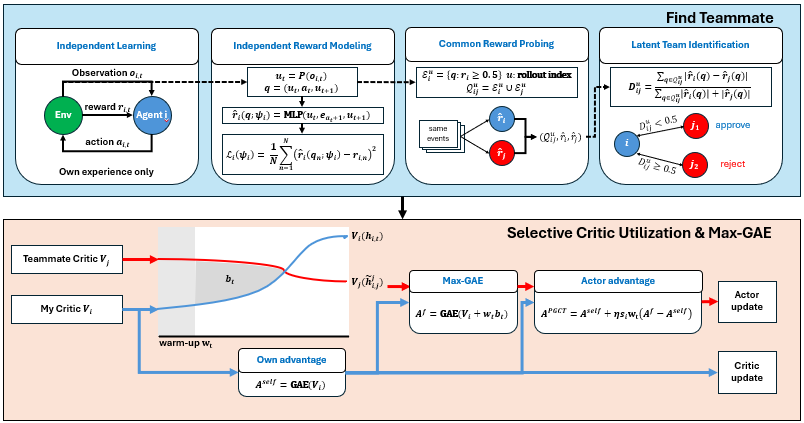
\includegraphics[width=.97\textwidth]{../figures/fig_overall.png}
\caption{Overall PGCT procedure for agent $i$. Top: the agent learns from its own experience and fits a reward predictor on public transitions. When it meets a peer, both predictors answer the same reward-event probes, and the peer is approved if the response distance stays small (simplified; the full rule is Eq.~\ref{eq:approval}). Bottom: the Critic of an approved teammate raises the value input of GAE by the positive uplift $b_t$. This changes only the Actor update. The Critic keeps learning its own return. All computation is local, and peers exchange public event views, predicted responses and Critic weights only when they meet.}\label{fig:architecture}
\end{figure*}

Figure~\ref{fig:architecture} shows the two parts of PGCT: team discovery (top) and peer Critic access (bottom). Algorithm~\ref{alg:pgct} lists one update. Lines 1--14 are for Q1 and lines 15--20 for Q2.

\subsection{Individual Reward Prediction}
Each agent trains a multilayer perceptron to predict its own reward from public transitions $q=(u_t,a_t,u_{t+1})$:
\ModelEquation
Here $e_{a_t+1}$ is the one-hot vector of the action ($e_k$ is the $k$-th unit vector of $\mathbb R^{5}$, and actions are numbered from 0). An event is a transition with own reward $r_i\ge0.5$. Events are rare, so each agent keeps a separate buffer of its recent events and fills a fixed share of every training batch with them. For a batch $\{(q_n,r_{i,n})\}_{n=1}^{N}$, the loss is
\RewardLossEquation
The public view hides private information, so the same public transition can be rewarding at one time and not at another. The predictor then learns the expected reward of the transition, and this is the quantity we compare.

\subsection{Reward Probes}
When agents $i$ and $j$ have met in rollout $u$, they build a common probe set
\ProbeEquation
Here $\mathcal E_i^u$ holds the public views of the most recent own events of agent $i$, recorded before rollout $u$ starts. No reward value is part of a probe. If both agents have been rewarded, their events already contain the information that separates teams: a delivery at one goal is rewarding for one team but not for the other.

\paragraph{Snapshot at rollout start.}
A pair is compared at the end of a rollout, but it may have met early in the rollout. To use only information that existed at the time of contact, each agent freezes its event views, its maturity flag and its predictor at the start of the rollout. Predictors are refitted only after a rollout. The comparison uses the frozen state and is done before the refit.

\begin{figure}[t]
\centering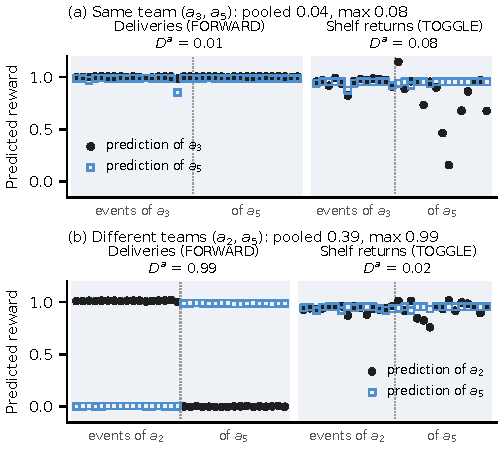
\includegraphics[width=\columnwidth]{../figures/fig_discovery_data.pdf}
\caption{Reward predictions of two agents on their common probes, from saved predictors of a real run (corner goals, individual rewards, seed 1, 4.35M steps; earlier-rule run, no mirrored probes). The probes are the 32 most recent own events of each agent, grouped by action. (a) Teammates $a_3$ and $a_5$ predict high reward on every probe. (b) Agents $a_2$ and $a_5$ of different teams agree on shelf returns, which reward both teams, but disagree on deliveries. Their pooled distance (0.39) is below the threshold 0.5, while the per-action maximum (0.99) is not.}\label{fig:discovery}
\end{figure}

\subsection{Response Distance and Team Discovery}
Both predictors are evaluated on the same probes (Figure~\ref{fig:discovery}). We group the probes by their action. Let $\mathcal Q_{ij}^{u,a}$ be the probes with action $a$ and $\mathcal E_i^u(a)$ the events of agent $i$ with action $a$. The response distance is
\ActionDistanceEquation
So a pair is compared on action $a$ only if each agent has at least $n_{\min}$ own events with this action. If no action qualifies, the pair is not compared in this round. If a denominator is below $10^{-8}$, that action is skipped.

Each per-action distance lies in $[0,1]$ by the triangle inequality and does not depend on a reward scale shared by both predictors. We take the maximum over actions for the following reason. If all probes are put together, the distance equals $\sum_a w_aD_{ij}^{u,a}$, where $w_a\ge0$ is the share of the denominator that comes from action $a$ and $\sum_a w_a=1$. This pooled distance is therefore never larger than the maximum, and the weight of an action grows with the predicted reward on it. An event that rewards every team, such as returning a shelf in our task, then gets a large weight and can hide a clear disagreement on another action (Figure~\ref{fig:discovery}b). Teammates have the same reward rule, so all their per-action distances are small, and the maximum is small as well. The condition on $n_{\min}$ prevents an agent from being judged on events it has rarely been rewarded for.

An agent is \emph{mature} ($m_i^u=1$) if it has seen at least 20 own events, its predictor has been fitted, and its mean prediction on its own recent events is at least 0.3. Pairs are compared every five updates and only if both agents are mature. The distance is smoothed over comparison rounds, and the pair is approved by
\ApprovalEquation
Here $n_{ij}$ counts the rounds that use new predictors: a round is counted only if $\widehat r_i$ or $\widehat r_j$ was refitted since the last counted round of the pair. Rounds without a refit change neither $\bar D_{ij}$ nor $n_{ij}$. The approval is symmetric. It is kept when the agents lose contact, but it is used only when they meet again. The threshold 0.5 is fixed in advance. No team label is used in this decision.

Discovery is possible only if the reward rules of two teams give different predictions on some public events. With the per-action distance, this difference must appear in an action that both agents have experienced at least $n_{\min}$ times. An agent that has never been rewarded has no prediction to compare, so PGCT abstains for it.

\subsection{Peer Critic Access}
The donor set of agent $i$ in rollout $u$ is
\begin{equation}\label{eq:donorset}
\mathcal G_i^u=\{j\ne i: C_{ij}^u=1,\ B_{ij}=1\}.
\end{equation}
Donor Critic weights are the weights used during rollout $u$. They are received on contact and are not changed during the update. Agent $i$ runs its own observation sequence through each donor Critic, so the donor's recurrent state is computed by the receiver and never sent. This replay starts from a zero state at the start of the rollout and is reset at episode ends. The first few replayed values are not reliable yet, so a mask $w_t=0$ removes them.

\begin{algorithm}[tb]
\caption{PGCT update $u$ of agent $i$}
\label{alg:pgct}
\begin{algorithmic}[1]
\REQUIRE Actor $\pi_{\theta_i}$, Critic $V_i$, reward predictor $\widehat r_i$, pair statistics $\bar D_{ij},n_{ij}$
\STATE Freeze $\mathcal E_i^u$, $m_i^u$, $\widehat r_i^{\,u}$ \COMMENT{rollout-start snapshot}
\STATE Roll out $\pi_{\theta_i}$; store $(q_t,r_{i,t})$; add $q_t$ to the events if $r_{i,t}\ge0.5$
\STATE Record contacts $C_{ij}^u$ \COMMENT{Eq.~\ref{eq:donor}}
\IF{$u \bmod 5=0$}
\FOR{each $j$ with $C_{ij}^u=1$ and $m_i^u=m_j^u=1$}
\STATE $\mathcal Q_{ij}^u\leftarrow\mathcal E_i^u\cup\mathcal E_j^u$
\STATE $D_{ij}^u\leftarrow\max_{a\in\mathcal A_{ij}^u}D_{ij}^{u,a}$ \COMMENT{Eq.~\ref{eq:distance}}
\IF{$\widehat r_i$ or $\widehat r_j$ was refitted since the last counted round}
\STATE $\bar D_{ij}\leftarrow(1-\beta)\bar D_{ij}+\beta D_{ij}^u$,\ \ $n_{ij}\leftarrow n_{ij}+1$
\ENDIF
\STATE $B_{ij}\leftarrow\mathbf 1[n_{ij}\ge3,\ \bar D_{ij}<0.5]$ \COMMENT{Eq.~\ref{eq:approval}}
\ENDFOR
\STATE Refit $\widehat r_i$ by minimizing $\mathcal L_i^r$ \COMMENT{Eq.~\ref{eq:rloss}}
\ENDIF
\STATE $\mathcal G_i^u\leftarrow\{j:C_{ij}^u=1,\ B_{ij}=1\}$
\STATE $b_{i,t}\leftarrow[\max_{j\in\mathcal G_i^u}V_j(\tilde h_{i,t}^{\,j})-V_i(h_{i,t})]_+$ \COMMENT{Eq.~\ref{eq:max}}
\STATE $f_{i,t}\leftarrow V_i(h_{i,t})+w_tb_{i,t}$
\STATE $A^{f}\leftarrow\mathrm{GAE}(f)$,\ \ $A^{\rm self}\leftarrow\mathrm{GAE}(V_i)$ \COMMENT{Eq.~\ref{eq:gae}}
\STATE $A^{\rm PGCT}_{i,t}\leftarrow A^{\rm self}_{i,t}+\eta s_iw_t(A^f_{i,t}-A^{\rm self}_{i,t})$ \COMMENT{Eq.~\ref{eq:blend}}
\STATE Update $\pi_{\theta_i}$ with $A^{\rm PGCT}$ and $V_i$ toward $R^{\rm self}$ \COMMENT{Eq.~\ref{eq:ppo}}
\end{algorithmic}
\end{algorithm}

\subsection{Max-GAE Advantage Estimation}
For a nonempty donor set, the positive uplift and the combined value are
\MaxEquation
GAE uses the trainer's handling of episode ends and time limits:
\GAEEquation
where $d_t$ marks episode ends and $z^f_{i,t}$ is the value of a captured time-limit observation (zero otherwise). The self advantage $A^{\rm self}$ uses the same recursion with $V_i$ instead of $f$. The Actor advantage is
\BlendEquation
The mask $w_t$ multiplies the whole difference $A^f-A^{\rm self}$, not only $b$. If only $b$ were masked, uplift from later steps could still enter the masked steps through the GAE recursion. The factor $s_i\le1$ reduces a large auxiliary term to the scale of the agent's own advantage, but it never increases a small one. In our task, the raw difference was 2.6--12 times $\operatorname{std}(A^{\rm self})$ for lagging agents. Without $s_i$, PPO's advantage normalization (Eq.~\ref{eq:ppo}) would make the result almost independent of $\eta$. If no donor is approved or the uplift is zero at every step, $A^{\rm PGCT}=A^{\rm self}$, so the method reduces to independent PPO.

\subsection{Actor and Critic Updates}
The Actor is trained by PPO with $A^{\rm PGCT}$ in place of the usual advantage $A^{\rm self}$. As in standard PPO, the advantage is first normalized for each agent over the rollout:
\PPOEquation
The Actor maximizes $L_i^\pi$ plus an entropy bonus. The Critic is trained as in independent PPO. Its target $R^{\rm self}$ is computed from $A^{\rm self}$, not from $A^{\rm PGCT}$, and it minimizes the clipped value loss toward this target. Peer Critics therefore change only the Actor update, and there is no peer distillation loss. The Actor and Critic have separate encoders and recurrent layers. They share one gradient-norm clip, so the Actor advantage can change the size of a Critic step but not its target.

\section{Experiments}
\begin{figure*}[t]\centering
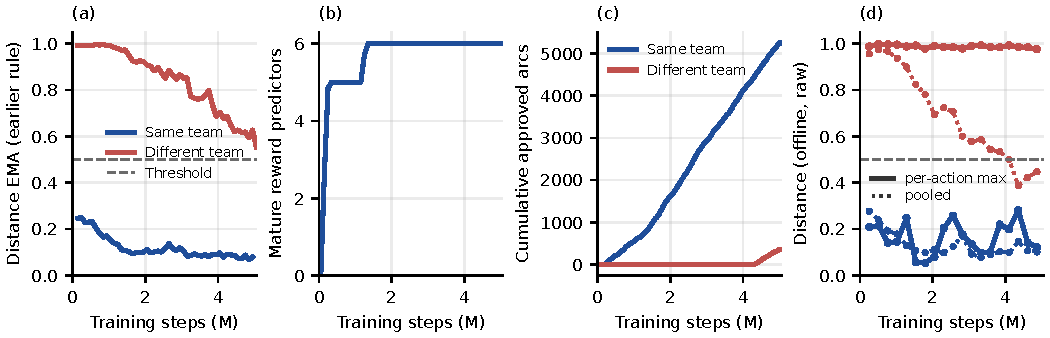
\includegraphics[width=.98\textwidth]{../figures/discovery_log_v2.pdf}
\caption{Discovery in the warehouse task (corner goals, individual rewards, seed 1, 5M steps). (a)--(c) come from the training log of the earlier rule (pooled distance, mirrored probes, $r_c=3$). (a) Mean response-distance EMA of compared pairs in 100k-step bins; the dashed line is the approval threshold. (b) Number of agents with a mature reward predictor. (c) Cumulative directed peer-access arcs by true relation. (d) Raw distances recomputed offline from the saved predictors and probes of every checkpoint, without mirrored probes: the largest same-team value (blue) and the smallest different-team value (red), for the per-action maximum (solid) and the pooled distance (dotted).}\label{fig:gate-data}
\end{figure*}

\subsection{Setup}\label{sec:setup}
\paragraph{Environment.} We use a multi-team version of the robotic warehouse \cite{benchmark}. The grid has $11\times10$ cells, and six agents form two teams of three. The team goals are at the two bottom corners, $(0,10)$ and $(9,10)$, and each team has three requested shelves. Observations are semantic grids with sensor radius five. Every agent receives its own reward: 1 for a delivery, 1 for a shelf return, 0.15 for picking up a requested shelf, small progress terms (0.02, 0.005, 0.002) and small penalties (0.002--0.05) for unproductive actions. No team reward is used. Table~\ref{tab:settings} lists the learning settings.

\paragraph{Implementation.} The public view $P(o)$ keeps six ego features and eleven physical grid channels within radius two (281 values), so the predictor input has $281+5+281=567$ values. The predictor has two hidden layers with 128 and 64 ReLU units. Each agent stores its last 20{,}000 transitions and, separately, its last 512 events. Events are less than 0.5\% of all transitions, so a quarter of every batch comes from the event buffer. Every five PPO updates, the predictor takes 50 Adam steps (batch 256, learning rate $10^{-3}$). The probes use the 32 most recent events of each agent, and $n_{\min}=8$. The replay mask removes donor values until eight observations have passed or the first reset occurs.

\paragraph{Method versions.} The discovery results below come from an earlier version of the rule. It used the distance on all probes at once (pooled), added left--right mirrored copies of the probes, and used $r_c=3$. Section~\ref{sec:discovery} explains why we changed to the per-action distance. Runs of the current method (per-action distance, no mirrored probes, $r_c=5$) on a wider $11\times16$ map are in progress.

\begin{table}[t]\centering\small
\begin{tabular}{lr}\toprule
Setting & Value\\\midrule
Rollout / recurrent sequence & 1024 / 64 steps\\
PPO epochs / minibatches & 4 / 8\\
Learning rate / entropy & $2\times10^{-4}$ / 0.05\\
PPO clip / value clip & 0.2 / 0.2\\
Discount / GAE parameter & 0.99 / 0.95\\
Encoder / GRU width & 128 / 128\\
Reward fit: interval / steps & 5 updates / 50\\
Event threshold / maturity & $r\ge0.5$ / 20 events\\
Probe events per agent / $n_{\min}$ & 32 / 8\\
EMA $\beta$ / threshold / rounds & 0.35 / 0.5 / 3\\
Max-GAE $\eta$ / scale & 0.5 / shrink\\
Earlier runs: $r_c$ / mirrored probes & 3 / yes\\\bottomrule
\end{tabular}
\caption{Environment interaction and PGCT settings.}\label{tab:settings}
\end{table}

\paragraph{Branch runs.} To run the complete method online, we start from a common independent-PPO checkpoint at 1.024M steps (seed 1) and train for 0.5M more steps with seeds 1, 3 and 5. These seeds keep the goal layout of the checkpoint. At this checkpoint, three agents ($a_0,a_1,a_4$) deliver little or nothing. As a control, we run the same branches with true teammates as donors, restricted to agents with mature predictors. These runs log the same discovery statistics. Branch seeds continue one training run, so they are not independent training seeds.

\subsection{Team Discovery}\label{sec:discovery}
Figure~\ref{fig:gate-data} shows a 5M-step run (seed 1) with the earlier discovery rule. Same-team and different-team pairs separate as soon as agents become mature. In the 0.1--0.25M bin, the mean response distance is 0.25 for teammates and 0.99 for other pairs, and five of six agents are mature by 0.25M. The same-team distance keeps falling (0.08 after 4M). The different-team distance stays near 0.99 until about 1M steps and then slowly decreases. Over the run, 5{,}252 directed peer-access arcs went to true teammates and 352 went to agents of the other team, which is a same-team share of 93.7\%. The first different-team approval appears at 4.28M steps, so all access before that point was correct. This share counts how often access was used, so it is not a pair-level accuracy. The run used positions at the end of an update as contacts and an earlier peer-usage rule, so it evaluates only the discovery part.

We found the cause of the late decrease. Both teams are rewarded for returning a shelf, and the public view of a return looks the same for both teams. As agents learned to finish delivery-and-return cycles, returns grew from about 3 to about 14 of the 32 recent events of active agents, and both predictors gave them high reward. The pooled distance then fell below 0.5 for the three pairs between the most active agent and the other team, and these three pairs produced all 352 different-team arcs. This is why we now use the per-action distance. We recomputed both distances offline from the saved predictors and probes of 25 checkpoints (this run and three branch runs), without mirrored probes. With the per-action distance, teammates were at most 0.28 and other pairs at least 0.97 at every checkpoint. With the pooled distance, one different-team pair reached 0.39 (Figure~\ref{fig:gate-data}d).

As a further offline check, we replayed a subsample of the experience of a finished independent-PPO run (0.26--5M steps, about 1/180 of its transitions) through the earlier rule, assuming that every pair is in contact in every round. Of the 15 pairs, the 10 pairs that reached a decision were all classified correctly: four same-team approvals and no different-team approval (same-team distances 0.14--0.18, different-team 0.58--0.70). The other five pairs all involved the one agent that never learned to deliver, and they abstained. Removing the mirrored probes from this replay did not change any decision.

The branch runs (Section~\ref{sec:setup}) execute the complete method online, with rollout-start snapshots and the contact rule. In the three PGCT branches (seeds 1, 3 and 5; seed 5 up to 0.46M of its 0.5M steps), no different-team pair was ever approved, and all donor arcs used by Max-GAE went to true teammates (1{,}920, 1{,}350 and 1{,}258). The first approval came 20k--26k steps after branching. Four agents became mature in each run: all three agents of one team and one agent of the other team. PGCT approved all six directed arcs inside the first team. It approved none of the six arcs between the single mature agent and that team. So it found 6 of the 12 same-team arcs and abstained on the rest. The three control runs also show no different-team approval. These branches cover 1.02--1.52M training steps, before the late decrease of the different-team distance in the 5M run.

\subsection{Why the Team Relation Matters for Peer Values}
\begin{figure}[t]
\centering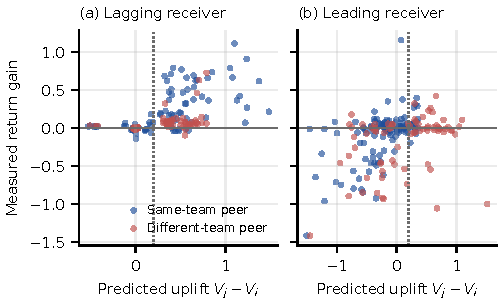
\includegraphics[width=\columnwidth]{../figures/counterfactual.pdf}
\caption{Counterfactual check on saved independent-PPO checkpoints (four datasets). No agent is trained with Max-GAE here. The check asks whether the uplift that Max-GAE would add matches a real gain. Each point is one state of a receiver. The x-axis is the uplift $V_j-V_i$ that a peer's Critic predicts for the receiver. The y-axis is the measured change of the receiver's own return over 100 steps when it acts with the peer's policy (8 repetitions with common random numbers). (a) Lagging receivers. (b) Leading receivers. The dotted line marks an uplift of 0.2.}\label{fig:cf}
\end{figure}

We checked whether a teammate's Critic is more useful than the Critic of another team. We used saved checkpoints of independent PPO: two time points of one run and two runs of an earlier configuration with visible coordinates. From the same environment state, a receiver acted either with its own policy or with a peer's policy, while all other agents kept their own policies. We then compared the change of the receiver's own return with the uplift that the peer's Critic predicted (Figure~\ref{fig:cf}). For lagging receivers with a predicted uplift above 0.2, same-team peers increased the return in 89\% of 56 cases, by 0.36 on average. Different-team peers with similar predicted uplifts gave only 0.10 on average. For leading receivers, different-team uplifts above 0.2 came with an average change of $-0.04$, and only half of them increased the return. The predicted uplift was also up to 1.6 times larger than the real gain. These results support both the discovery step and the scaling of the uplift.

\section{Conclusion}
PGCT finds latent teammates online from individual reward responses. Each agent predicts its own reward, compares its predictions with those of the peers it meets on public reward events, action by action, and approves a peer only after repeated agreement backed by enough own experience. Approved teammates' Critics change the Actor advantage through a masked and scaled Max-GAE term, and each Critic keeps its own return. In a two-team warehouse, discovery separated teammates early and sent most peer access to true teammates. In branch runs of the complete method, no different-team pair was approved. We are still testing whether this access speeds up learning.

%% The file named.bst is a bibliography style file for BibTeX 0.99c
\bibliographystyle{named}
\bibliography{../references}

\end{document}
